\chapter{Trabalhos Relacionados} \label{cap:cap3}

Os trabalhos apresentados neste capítulo vão desde abordagens de simulação de procedimentos de anestesia usando \textit{phantons} a simuladores computacionais. É interessante destacar que alguns simuladores computacionais são híbridos no sentido de que usam \textit{phantoms} como parte do processo de simulação. Apresentamos ao final um comparativo descrevendo a nossa abordagem frente aos principais benefícios de cada abordagem estudada.  

\textcite{Vaughan2013} citam trinta e um simuladores (entre computacionais e com uso de \textit{phantoms}). Destes, dezesseis são apenas epidurais, nove que permitem tanto a punção epidural quanto a raquidiana e seis apenas raquidianos. São discutidas as limitações e vantagens de cada um, de forma a identificar características desejáveis para serem incluídas em um simulador. 

No trabalho de \textcite{Isaacs2015} os autores citam uma pesquisa onde também são elencadas diversas características interessantes para um simulador epidural. Dentre os itens com mais relevância citados por \textcite{Isaacs2015} estão: coluna fisicamente palpável, representação da técnica de perda de resistência (do inglês inglês Lost of Resistence, \acrshort{LoR}) de forma realista (para solução salina e ar), ajuste da posição do paciente, mapeamento de características do paciente (obesidade, gravidez), \textit{feedback} a respeito da correta execução.

A principal vantagem dos modelos com uso de \textit{phantoms} é a presença física do manequim que representa o paciente. Uma das principais desvantagens é a dificuldade na variabilidade de cenários (pacientes) distintos. Outra desvantagem é a dificuldade na representação da diferença existente entre a resistência dos tecidos biológicos e os tecidos nos quais os modelos físicos são constituídos (usualmente borracha e plástico).

Os dispositivos hápticos têm evoluído muito ao longo dos últimos anos. Os modelos computacionais com hápticos têm como pontos a favor a versatilidade. As possibilidades computacionais da tecnologia háptica e as visualizações 3D de tempo real são outros pontos positivos associados a esta tecnologia. 
Soluções computacionais podem criar um modelo de forças de inserção da agulha. Para este fim pode-se usar como base as medições das forças aplicadas para inserção de agulhas em animais considerados próximos dos humanos, assim como em cadáveres e até mesmo voluntários reais \cite{Hiemenz1998, Holton2001,Langton1990,McKay2010,Naemura2009,Tran2009,Vaughan2012}. Estes modelos podem contemplar uma grande variabilidade de cenários através de ajustes de parâmetros. 

A seguir serão apresentados os simuladores de punções mais completos. Primeiro os que somente fazem uso de \textit{phantoms}, em seguida os que usam de ferramentas computacionais.  

\section{Simuladores que só usam \textit{phantoms}} \label{sec:SimuladoresPhantoms}

Os simuladores baseados em \textit{phantoms} (ou manequins) mais completos são discutidos aqui com suas principais características. As características positivas devem idealmente ser contempladas ou até melhoradas em novos simuladores. Todas as soluções listadas estão disponíveis atualmente. Elas permitem ao menos a simulação da anestesia peridural, possuem a coluna fisicamente palpável e permitem a escolha do ponto e ângulo de inserção da agulha. Todos esses trabalhos permitem que o procedimento seja feito com o paciente sentado ou deitado e o escoamento do fluido cérebro espinhal é simulado ao perfurar a dura-máter. É possível escolher o ponto de inserção em todos estes simuladores.

A solução \textit{SimULab Lumbar Epidural Trainer} possui até 4 variações de pacientes (normal, idoso e obeso e obeso idoso). A Figura \ref{fig:simuladorSimulab} ilustra o uso deste simulador. O material deste manequim foi produzido de forma a permitir o uso deste equipamento \cite{SimulabCorporation2008}. Este simulador permite somente a anestesia epidural e foi incluído aqui por que esta anestesia possui algumas similaridades com as anestesias raquidianas. 

\begin{figure}[ht!]
    \centering
        \begin{tabular}{cc}
        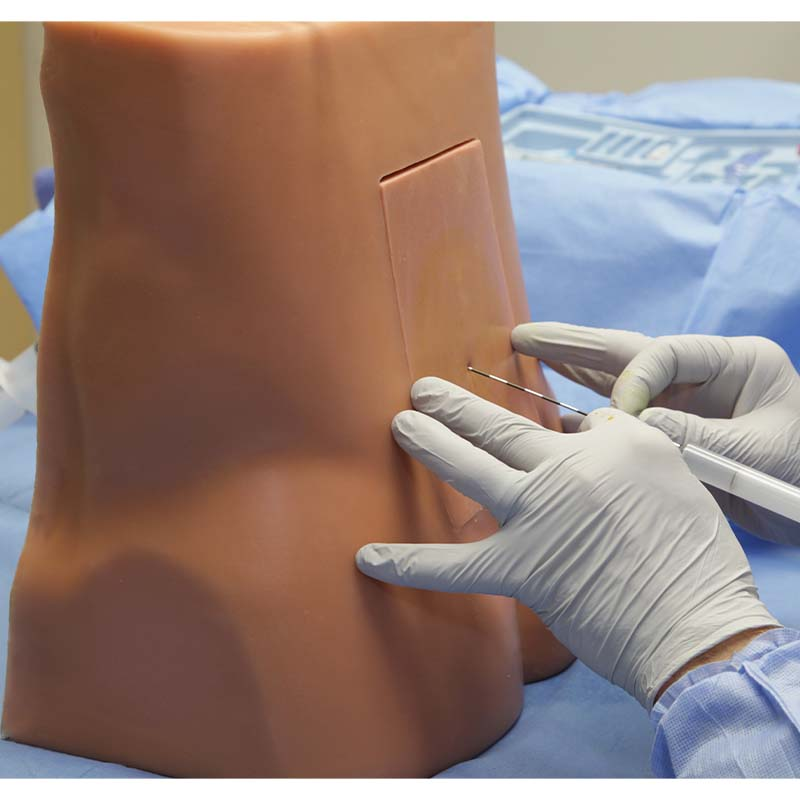
\includegraphics[width=0.3\linewidth]{capitulos/figuras/simulab-insercao-agulha.jpg} & 
        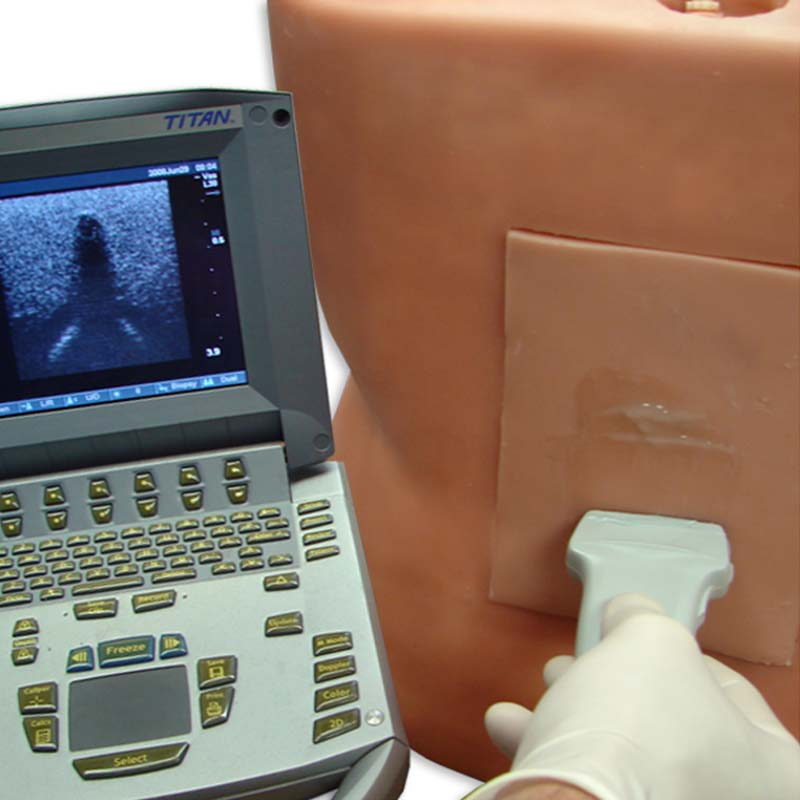
\includegraphics[width=0.3\linewidth]{capitulos/figuras/simulab-ultrassom.jpg} 
        \\
        (a) & (b)
        \end{tabular}
    \caption{Demonstração de uso do simulador SimULab Lumbar Epidural Trainer \cite{SimulabCorporation2008}: (a) Inserção da agulha (b) Exame de ultrassom.}
    \label{fig:simuladorSimulab}
\end{figure}

O simulador \textit{Nasco Life/form® Spinal Injection Sim} permite treinamentos nos dois tipos principais das anestesias regionais. As vértebras L1 e L2 ficam visíveis externas ao corpo simulado pelo manequim como pode ser visto na Figura \ref{fig:nascoSimulator}. Ele somente permite a punção entre as vértebras L3 até L5 \cite{Nasco2008}. 

\begin{figure}[ht!]
    \centering
    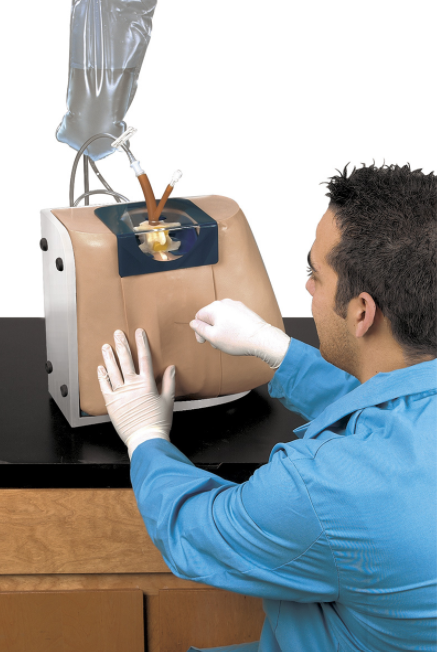
\includegraphics[width=0.3\linewidth]{capitulos/figuras/nascoSimulator.png} 
    \caption{Demonstração de uso do simulador \textit{Nasco Life/form® Spinal Injection Sim} \cite{Nasco2008}.}
    \label{fig:nascoSimulator}
\end{figure}

O \textit{Blue Phantom Lumbar Puncture and Spinal Epidural} (Figura \ref{fig:bluePhantom}) também foi produzido em material que possibilita o uso do ultrassom. Este simulador possui somente duas opções de variação de pacientes (normal e obeso) e possibilita tanto anestesias epidurais como raquidianas \cite{BluePhantom2011}. 

\begin{figure}[ht!]
    \centering
        \begin{tabular}{ccc}
        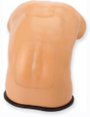
\includegraphics[width=0.17\linewidth]{capitulos/figuras/BluePhatom-manequim.png} & 
        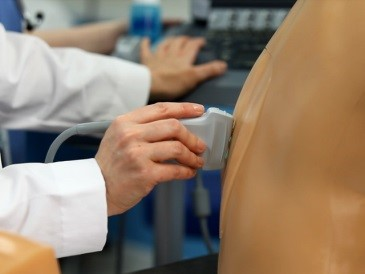
\includegraphics[width=0.3\linewidth]{capitulos/figuras/BluePhatom-ultrassom.jpg} 
        &
        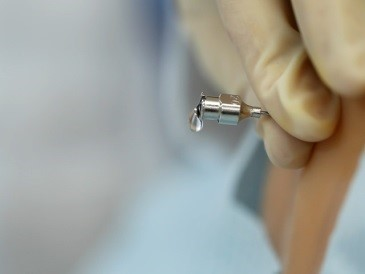
\includegraphics[width=0.3\linewidth]{capitulos/figuras/BluePhatom-escorrimentoLiquor.jpg} 
        \\
        (a) & (b) & (c)
        \end{tabular}
    \caption{Blue Phantom Lumbar Puncture and Spinal Epidural \cite{BluePhantom2011}: (a) Manequim (b) Uso do ultrasssom (c) Escorrimento do líquor do manequim.}
    \label{fig:bluePhantom}
\end{figure}

S411 \textit{Lumbar Puncture Trainer} é outro simulador de anestesias regionais que pode ser observado na Figura \ref{fig:simuladorS411}. Possui parte substituível vendida em separado que dura, segundo o fabricante, entre 15 e 25 usos dependendo da espessura da agulha usada nas simulações. As vértebras representadas vão da L2 até a L5 mas possibilita a punção entre a L4 e L5 ou L3 e L4. Só permite a inserção da agulha entre vértebras. Só apresenta variações de cor do manequim não representado diferentes classes de pacientes \cite{GaumardScientific}. Um exemplo de video mostrando seu uso pode ser visto no link\footnote{\url{https://youtu.be/O77\_UWo0JSc}}.

\begin{figure}[ht!]
    \centering
        \begin{tabular}{cc}
        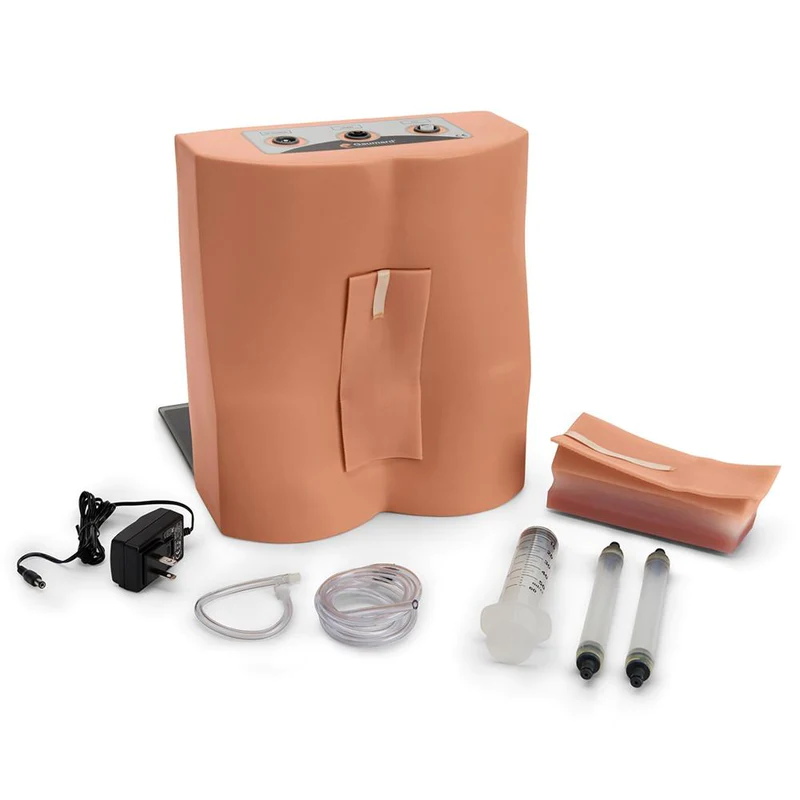
\includegraphics[width=0.3\linewidth]{capitulos/figuras/S411-Lumbar Puncture Trainer Kit.png} & 
        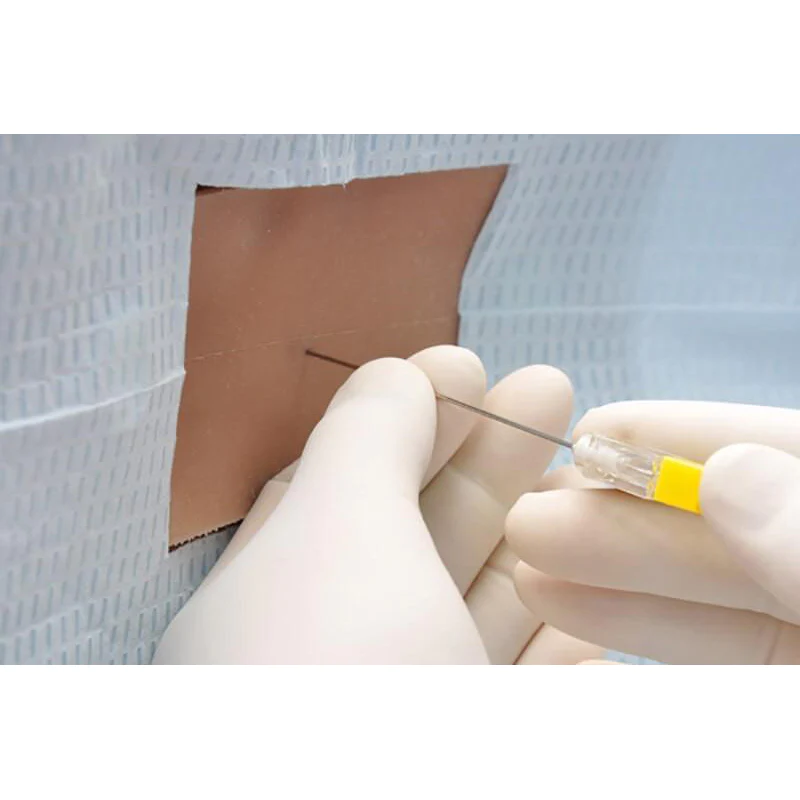
\includegraphics[width=0.3\linewidth]{capitulos/figuras/S411-Lumbar Puncture Trainer Needle.png} 
        \\
        (a) & (b)
        \end{tabular}
    \caption{Demonstração do simulador S411 Lumbar Puncture Trainer \cite{GaumardScientific}: (a) Kit (b) Inserção da agulha.}
    \label{fig:simuladorS411}
\end{figure}

Outro simulador que também possibilita anestesias epidurais e raquidianas é o M43E \textit{Ultrasound Compatible Lumbar Puncturee/Epidural Simulator}. Ele possui 4 variações de pacientes (normal, obeso, idoso e idoso obeso) e possibilita o uso ultrassom como demostrado na Figura \ref{fig:M43ESimulator} . Uma limitação deste é somente apresentar as vértebras L2 até L5 \cite{KyotoKagaku2015}mas como vimos anteriormente, na seção \ref{sec:anestesiaRaquidiana}, estas são as vértebras mais comuns para anestesia raquidiana.

\begin{figure}[ht!]
    \centering
    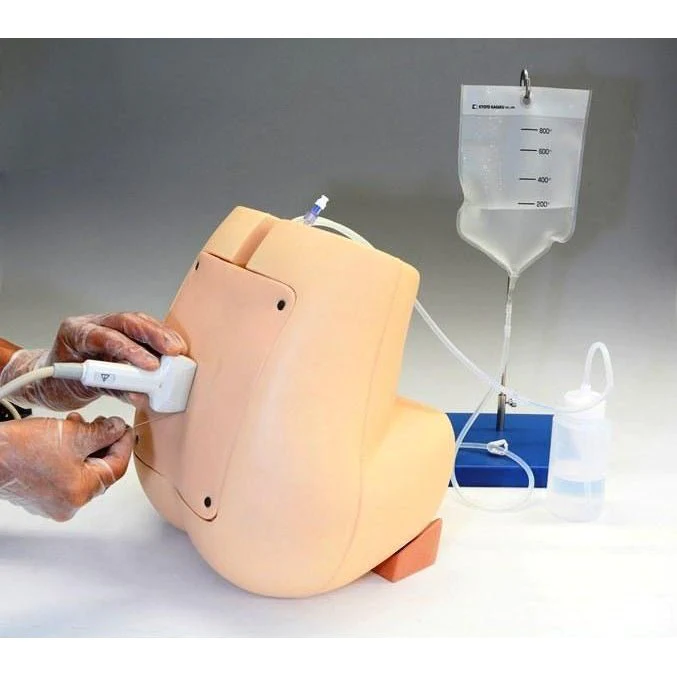
\includegraphics[width=0.3\linewidth]{capitulos/figuras/M43E Simulator.png} 
    \caption{M43E \textit{Ultrasound Compatible Lumbar Puncture/Epidural Simulator} \cite{KyotoKagaku2015}.}
    \label{fig:M43ESimulator}
\end{figure}

\texxtcite{Mashari2018} testou o uso de um manequim de baixo custo impresso em impressora 3D com material que permite o uso de ultrassom. No teste ele foi comparado por 21 anestesistas com o modelo de paciente normal do simulador comercial \textit{SimULab Lumbar Epidural Trainer}. As respostas dos participantes demonstraram resultados comparáveis tendo avaliações mais baixas somente no teste da apalpação. O modelo impresso foi criado a partir de imagens de \acrshort{TC} segmentadas e posteriormente modeladas pelos autores. Este modelo carece de variabilidade, pois simula apenas um modelo de corpo para cada manequim impresso. Esta variabilidade pode ser obtida com um trabalho de obtenção, segmentação e modelagem de diversas imagens médicas referentes a pacientes com características físicas distintas.

A Tabela \ref{tab:comparacaoSimuladoresPhantoms} resume uma série de características importantes destes simuladores. Durante as pesquisas encontramos outros simuladores que não foram descritos aqui por possuírem  características muitos similares ou serem menos abrangentes dos mencionados aqui.

\begin{table}[!ht]
\begin{center}
\caption{Comparação dos simuladores baseados em \textit{phantoms}.}
\label{tab:comparacaoSimuladoresPhantoms}
%\begin{tabular}{|p{0.27\linewidth}|p{0.55\linewidth}|p{0.105\linewidth}|}
\begin{tabular}{|c|c|c|c|c|c|c|c|c|}
\hline
  Nome do simulador & 
  \rotatebox{90}{Ano de desenvolvimento} & 
  \rotatebox{90}{Epidural (E) Raquianestesia (R)} & 
  \rotatebox{90}{Testado por especialistas} & 
  \rotatebox{90}{Permite o uso de ultrassom} & 
  \rotatebox{90}{Variabilidade de pacientes} & 
  \rotatebox{90}{Coluna palpável} & 
  \rotatebox{90}{Escolha do ponto de inserção da agulha }  & 
  \rotatebox{90}{Abordagens mediana (M) e paramediana (P)} \\
\hline\hline
 SimULab Lumbar Epidural Trainer & 2008 & ER & N & S & 4 & S & S & MP \\
 Nasco Life/form® Spinal Injection Sim & 2008 & ER & N & N & 3 & S & S & MP \\
 {\begin{tabular}[c]{@{}c@{}}Blue Phantom Lumbar Puncture\\ and Spinal Epidural\end{tabular}} & 2011 & ER & N & S & 2 & S & S & MP \\
 S411 Lumbar Puncture Trainer & 2011 & ER & N & N & 1 & S & S & M\\
 \begin{tabular}[c]{@{}c@{}}M43E Ultrasound Compatible Lumbar\\ Puncture/Epidural Simulator\end{tabular}} & 2015 & ER & S & S & 4 & S & S & MP \\
 Manequim de baixo custo de Mashari & 2018 & ER & S & S & 4 & S & S & MP \\
\hline
\end{tabular}
\end{center}
\end{table}

\section {Simuladores computacionais}
\label{sec:simuladoresComputacionais}

Esta seção comenta os simuladores computacionais que possuem as características mais relevantes ao desenvolvimento das respostas conduzidas por computador à manipulação dos hápticos. 

O primeiro simulador epidural computacional, Epidural Sim \cite{Stredney1996} apresentou uma série de características interessantes. A representação do corpo do paciente em 3D teve as alterações das características de seus elementos obtida através de exames de \acrfull{RM}. Permite o uso de uma agulha real ligada a um dispositivo háptico. O modelo de forças foi baseado em medidas feitas durante inserções epidurais em porcos e cães combinados com opiniões de especialistas. Este simulador permite ainda a escolha do ponto de inserção da agulha assim como o seu ângulo. É disponibilizada uma interface de voz, o que possibilitava ser iniciado por comandos de voz do usuário assim como receber \textit{feedbacks} gerados pelo computador. A palpação da coluna não está disponível neste simulador. Chegou a ser testado por anestesistas que o consideraram muito mecânico, porém com potencial de melhora a partir de ajustes. Uma imagem do uso deste simulador pode ser vista na Figura \ref{fig:epiduralSim}. 

\begin{figure}[ht!]
    \centering
    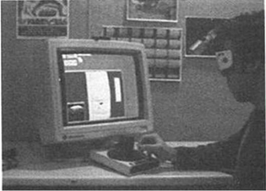
\includegraphics[width=0.3\linewidth]{capitulos/figuras/epiduralSimulator.png} 
    \caption{Epidural Sim em uso \cite{Stredney1996}.}
    \label{fig:epiduralSim}
\end{figure}

O único simulador computacional de punção lombar estudado que possibilita a palpação da coluna é o \textit{Epidural Injection Simulator, EIS} \cite{Wilson2003}. Esta característica é atendida através de um equipamento físico que fica conectado a uma unidade de controle. O simulador possui uma interface gráfica que mostra, em tempo real, a progressão da agulha em cada camada de tecido conforme ela é inserida. Existem 6 variações de pacientes e um \textit{feedback} de forças configurável. O dispositivo háptico usado aqui foi desenvolvido para este simulador, não sendo uma solução pronta de mercado. Não é permitida a escolha do ponto de inserção da agulha nem o seu ângulo de inserção, que são fixos. Uma nova versão deste simulador foi desenvolvida com o nome de \textit{Epidural Injection Simulator Profile Manager}. Essa, além das funcionalidades do seu antecessor possibilita a criação de cenários customizados de pacientes além das 6 opções pré-configuradas. Estas customizações podem inclusive ser salvas para uso posterior. O \textit{feedback} em tempo real nesta nova versão pode ser visualizada no monitor do computador na forma de gráficos \cite{CPRSavers&FirstAidSupply2018}. A Figura \ref{fig:EpiduralInjectionSimulator} exibe o visual do \textit{Epidural Injection Simulator Profile Manager} e do seu antecessor EIS que foi descontinuado com o lançamento da nova versão.

\begin{figure}[ht!]
    \centering
        \begin{tabular}{cc}
        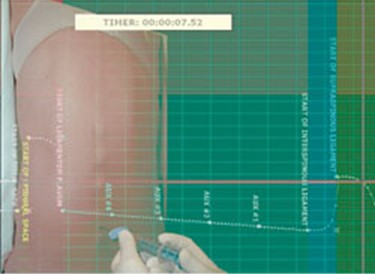
\includegraphics[width=0.4\linewidth]{capitulos/figuras/epiduralInjectionSimulatorPM.jpg} & 
        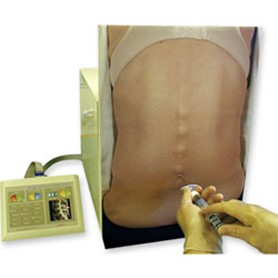
\includegraphics[width=0.3\linewidth]{capitulos/figuras/epiduralInjectionSimulator.jpg} 
        \\
        (a) & (b)
        \end{tabular}
    \caption{Imagens de exemplo das duas versões do \textit{Epidural Injection Simulator}: (a) \textit{Versão mais nova: Profile Manager} (b) Versão antiga: EIS (descontinuado)  \cite{CPRSavers&FirstAidSupply2018}.}
    \label{fig:EpiduralInjectionSimulator}
\end{figure}

Em 2006 foi lançado o \textit{Mediseus® epidural simulator} (MedicVision Pty Ltd, Melbourne, Austrália). Este simulador apesar de ter sido descontinuado apresentava algumas características interessantes como a exibição completa do corpo permitindo rotações e zoom \cite{Mayooran2006}. A pele pode ser tornada transparente tornando visíveis as cinco vértebras modeladas. Este simulador usa um \textit{Phantom Omni} dentro de uma caixa patenteada \cite{Brien2007} para o \textit{feedback} das forças na agulha incluindo a medida da pressão de ar na seringa. A agulha é movimentada na tela em tempo real assim que o dispositivo é utilizado pelo profissional em treinamento. O dispositivo pode ser conectado em qualquer laptop. Em uma avaliação feita sobre este simulador de 2007 \cite{Elks2007} ele não teve um bom retorno por parte dos anestesistas. O item com pior avaliação foi a sensação de LOR que somente 54\% dos especialistas julgaram como realista. Em um estudo posterior \cite{Lee2012} essa técnica foi avaliada com nota 4,7 de um valor máximo de 5 o que supõe uma representação próxima da sensação real esperada, já a simulação dos ossos nessa mesma avaliação recebeu nota 2,3 enquanto a do ligamento amarelo foi avaliado com nota 3,5. Na avaliação feita por \textcite{Lee2012} a nota 1 indicava uma representação muito pobre ou sem utilidade enquanto a nota 5 indica algo excelente ou muito útil. Uma imagem deste simulador pode ser vista na Figura \ref{fig:mediseusSimulator}.

\begin{figure}[ht!]
    \centering
    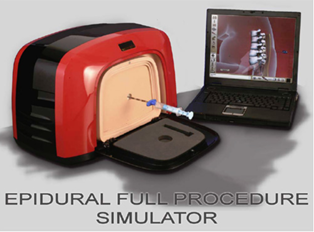
\includegraphics[width=0.6\linewidth]{capitulos/figuras/mediseusSimulator.png} 
    \caption{Aparelho e visual do \textit{Mediseus® epidural simulator}  \cite{Mayooran2006}.}
    \label{fig:mediseusSimulator}
\end{figure}

O \textit{Spinal Anaesthesia Simulator} \cite{Albert2007,Dreifaldt2006}, faz o uso de um dispositivo háptico \textit{Phantom Premium} 1.0 em conjunto com óculos 3D (Figura \ref{fig:spinalAnestesiaSim}). Permite tanto a simulação da anestesia peridural como a raquidiana. O modelo das costas é feito a partir de uma combinação de imagens de \acrfull{TC} e de \acrshort{RM}. Existem vários níveis de dificuldade configuráveis além de ser possível alterar o nível de visibilidade da pele. É feita uma análise do usuário proporcionando um \textit{feedback} a ele do seu nível de aprendizado e as habilidades adquiridas nos vários níveis de dificuldade disponíveis.

\begin{figure}[ht!]
    \centering
    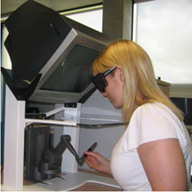
\includegraphics[width=0.3\linewidth]{capitulos/figuras/spinalAnestesiaSim.png} 
    \caption{Forma de uso do \textit{Spinal Anaesthesia Simulator}  \cite{Dreifaldt2006}.}
    \label{fig:spinalAnestesiaSim}
\end{figure}

O EpiSim \cite{YantricInc2011} foi desenvolvido em 2008. Ele faz uso do háptico \textit{Phantom Omni} além de um manequim e agulha epidural com uma seringa para recriar a sensação de perda de resistência. Só possui duas vértebras e um ponto fixo de inserção da agulha. A espessura de cada camada de tecido é configurável a partir da interface podendo estas configurações serem salvas para uso futuro. É dado um \textit{feedback} visual a partir de cores. Onde a cor verde indica o tecido atual e a vermelha indica possíveis toques no osso. Um som de aviso é ouvido no caso de perfuração da dura-máter. É possível efetuar a gravação da inserção de uma agulha inclusive com as forças empregadas para posterior exibição como outro tipo de \textit{feedback}. Esta etapa permite que um procedimento feito por especialistas seja visualizado em detalhes por profissionais inexperientes. A Figura \ref{fig:epiSim} ilustra este simulador.

\begin{figure}[ht!]
    \centering
    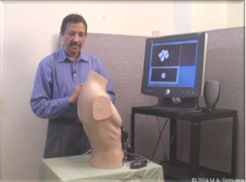
\includegraphics[width=0.4\linewidth]{capitulos/figuras/epiSim.png} 
    \caption{Imagem do simulador \textit{EpiSim} \cite{Frazzetto2011}.}
    \label{fig:epiSim}
\end{figure}

Um simulador de punção lombar criado por \textcite{Farber2008}  possui, além do dispositivo háptico \textit{Phantom Premium} 1.0, gráficos anatômicos e tela estereográfica. Os movimentos de rotação e em direção não perpendicular ao corpo do paciente são restritos quando a agulha está dentro do corpo \cite{Farber2008, Farber2009}. Uma abordagem de processamento de volume háptico descrita por \textcite{Lundin2005} foi adaptada para mapear as tomografias em forças. O paciente virtual 3D é construído a partir de dados de tomografia de pacientes reais e de dados do projeto \textit{Visible Human}. É importante ressaltar aqui que as imagens de tomografias não podem ser feitas com paciente com a coluna fletida que é a posição necessária para serem efetuada a raquianestesia (seja sentada ou deitada).  As visualizações incluem uma anatomia 3D e 3 visualizações 2D mostrando os cortes ortogonais (transversal, frontal e sagital). É possível usar uma visão sob a perspectiva da agulha virtual. A Figura \ref{fig:farberSimVisual} ilustra as opções de visualizações citadas, a visão da agulha aparece na parte superior esquerda. A visão pode ser rotacionada e amplificada por meio de zoom. A interface proporciona uma boa sensação e visão de  profundidade no corpo virtual através da visão estéreo. Possibilita a variação entre 3 opções de pacientes virtuais. Possui uma análise do percurso da agulha comparando esta com um caminho ótimo definido por especialistas e apresenta como \textit{feedback} ao usuário. Dá também retorno de perfuração de estruturas de risco bem como avalia o tempo de punção resultando numa nota geral de 0 a 100 calculada para comparar o sucesso dentre os usuários. Por fim é exibida para o usuário uma janela de \textit{feedback} onde é informado o desempenho e são apresentadas dicas de como melhorar a performance. Pelas diversas tecnologias envolvidas este simulador tem um custo consideravelmente maior que os demais. Na Figura \ref{fig:farberSimDispositivos} é possível visualizar os dispositivos envolvidos no uso do simulador. Testes num estudo piloto demonstraram que os médicos treinados neste simulador se saíram melhor do que os que não tiveram acesso a ele \cite{Farber2009}.

\begin{figure}[ht!]
    \centering
    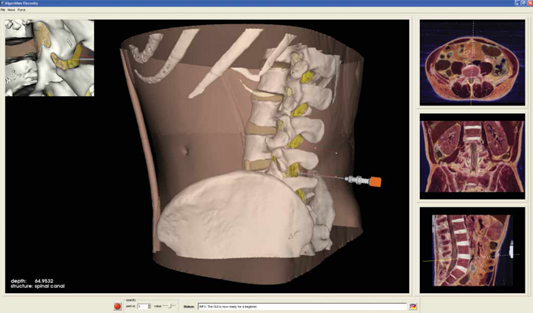
\includegraphics[width=0.8\linewidth]{capitulos/figuras/farberSimVisual.png} 
    \caption{Interface do simulador de punção lombar de \textcite{Farber2009} com opções de visualização 2D e 3D disponíveis.}
    \label{fig:farberSimVisual}
\end{figure}

\begin{figure}[ht!]
    \centering
    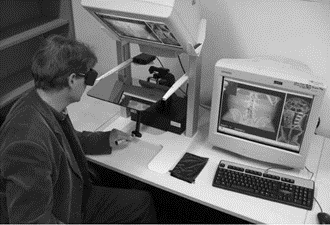
\includegraphics[width=0.5\linewidth]{capitulos/figuras/farberSimDispositivos.png} 
    \caption{Uso do simulador demonstrando os dispositivos utilizados \cite{Farber2009}.}
    \label{fig:farberSimDispositivos}
\end{figure}

\textcite{N.2013} criou e descreveu um simulador epidural que fez uso do háptico Novint Falcon e conectou uma seringa ao computador possibilitando a simulação da técnica de \acrshort{LoR}. A Figura \ref{fig:dubeySimSistema} ilustra uma tela de exemplo deste simulador que permite a variação de corpos via entrada de parâmetros. Possui simulação da apalpação para determinação do ponto de inserção da agulha e permite as duas abordagens de inserção da agulha. Cada vértebra desde a T2 até a L5 foi mapeada individualmente. O mapeamento das forças necessárias para perfuração e passagem da agulha pelas camadas foi feito através da medição das forças necessárias para execução destas atividades em cadáveres de porcos. Este simulador permite ainda a aplicação de transparência às camadas, o uso de rotação e zoom para melhor visualização de diferentes aspectos do corpo. Os autores não comentaram sobre \textit{feedback} para o usuário a respeito do seu desempenho somente do \textit{feedback} de forças na execução do procedimento.

\begin{figure}[ht!]
    \centering
    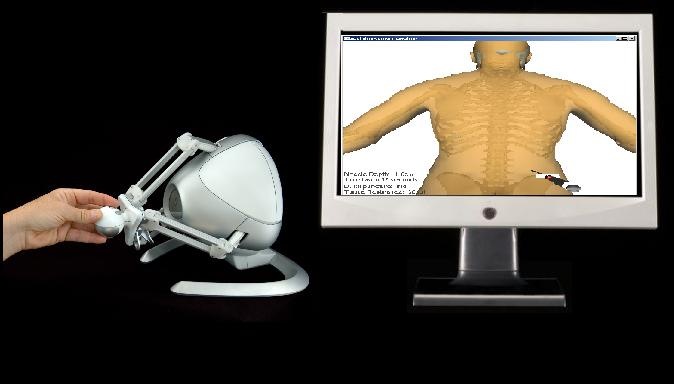
\includegraphics[width=0.5\linewidth]{capitulos/figuras/Dubey-ES-haptic-graphics.jpeg} 
    \caption{Exemplo de uso do simulador epidural de Dubey \cite{N.2013}.}
    \label{fig:dubeySimSistema}
\end{figure}

O \textit{Epidural Haptic Game Simulator}, EHGS \cite{Brazil2017}, utilizou um dispositivo háptico Phantom Omni e fez uso de elementos de jogos para trazer mais motivação para os usuários. Dentre os elementos de jogos estão presentes a divisão de etapas e atribuição de pontuação dada como \textit{feedback} para o usuário pela execução correta das tarefas envolvidas no procedimento de punção epidural. A simulação da técnica de LOR foi feita através da exibição de valores na tela ao clicar sobre um botão do háptico simulando o pressionamento do êmbolo da seringa. É possível escolher o ponto e ângulo de inserção da agulha. Não existe a opção de palpação da coluna para descoberta do local correto para efetuação da punção. Foi implementado um modelo de cálculo da espessura dos tecidos conforme peso, altura e idade do paciente de acordo com estudos em parturientes. A modelagem de forças de rigidez, atrito e corte necessárias para inserção e progresso da agulha nos tecidos foi desenvolvida com base em estudos destas forças para inserção de agulhas em tecidos de porcos e humanos. A ferramenta também disponibiliza uma forma manual de alteração destes parâmetros permitindo assim uma customização destas forças segundo as sensações do especialista. A Figura \ref{fig:brasilSimulator} mostra a interface do simulador EHGS em detalhes com o retorno de pontos obtidos, o tecido sendo perfurado no momento, a profundidade da ponta da agulha, as forças medidas e ângulo da agulha. É possível inserir a agulha na abordagem mediana e na paramediana porém, pela simplificação da modelagem das camadas, a agulha inserida na abordagem paramediana necessariamente irá perfurar as mesmas camadas da abordagem mediana o que não é o correto.  

\begin{figure}[ht!]
    \centering
    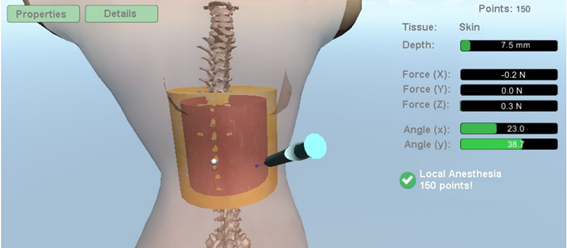
\includegraphics[width=0.8\linewidth]{capitulos/figuras/brasilSimulator.png} 
    \caption{Interface do simulador EHGS \cite{Brazil2017}.}
    \label{fig:brasilSimulator}
\end{figure}

No simulador epidural desenvolvido por \textcite{Senac2019} o objetivo principal foi a representação fiel das sensações durante a inserção da agulha incluindo a \acrshort{LoR} em detrimento da parte visual (o que pode ser observado na Figura \ref{fig:senacSim}). O ponto de entrada da agulha assim como as abordagens de inserção deste estavam portanto fora do escopo deste simulador. Ele foi testado por oito anestesistas (dois experientes e seis novatos). O foco foi na avaliação do nível de habilidade do usuário através da gravação do seu uso do simulador. Três tipos de paciente foram criados neste simulador (normal, obeso e calcificado). As dimensões dos pacientes foram configuradas a partir de imagens de \acrshort{RM} e as forças a partir do trabalho de \textcite{Tran2009}.

\begin{figure}[ht!]
    \centering
    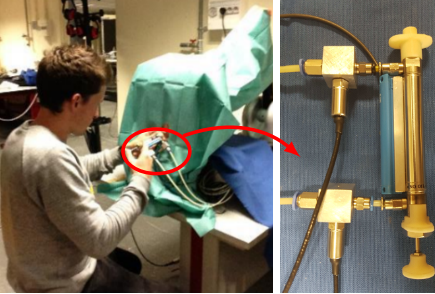
\includegraphics[width=0.6\linewidth]{capitulos/figuras/Senac-ES.png} 
    \caption{Interface do simulador Epidural de Senac \cite{Senac2019}.}
    \label{fig:senacSim}
\end{figure}

USEIT é o acrônimo em inglês do simulador epidural baseado em \textiti{Unity} para treinamento desenvolvido por \texcite{Moo-Young2021}. Os autores fizeram uso do dispositivo háptico \textiti{Novint Falcon} com uma customização para conexão da agulha epidural. Também desenvolveram uma customização adicional onde usaram Arduino e uma válvula manual de forma a simular o efeito de \acrshort{LoR} através da seringa. Estas duas customizações podem ser observadas na Figura \ref{fig:useitSim} que ilustra um usuário efetuando um procedimento no simulador. Apesar das customizações aumentarem o realismo na execução do procedimento, a existência delas impediu a inclusão da apalpação neste simulador. Os autores comentaram que para possibilitar a apalpação seria necessário aumentar a complexidade de montagem do sistema por parte dos usuários. O ambiente virtual remete a uma sala de operação como pode ser visto na Figura \ref{fig:useitSimAmbienteVirtual}. Nesta figura também fica claro que a aplicação de transparência nas camadas é possível neste simulador. O intestino delgado e os rins estão presentes no modelo 3D do paciente o que é um diferencial deste em relação aos demais simuladores porém os autores não comentam a possibilidade de variação de espessuras dos tecidos no modelo 3D do paciente. Como esta variabilidade não foi informada consideramos assumimos que o modelo é fixo e não adaptável. Como \textit{feedback} são apresentadas métricas de avaliação do desempenho após a simulação.

\begin{figure}[ht!]
    \centering
    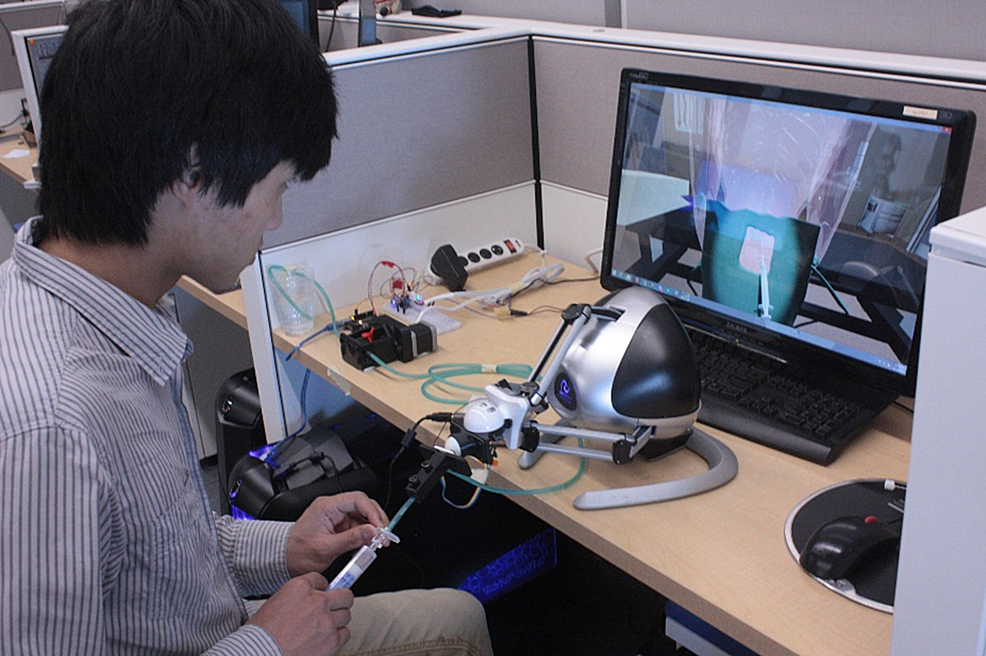
\includegraphics[width=0.7\linewidth]{capitulos/figuras/USEIT-uso.png} 
    \caption{Visão geral do uso do USEIT com as customizações visíveis \cite{Moo-Young2021}.}
    \label{fig:useitSim}
\end{figure}

\begin{figure}[ht!]
    \centering
    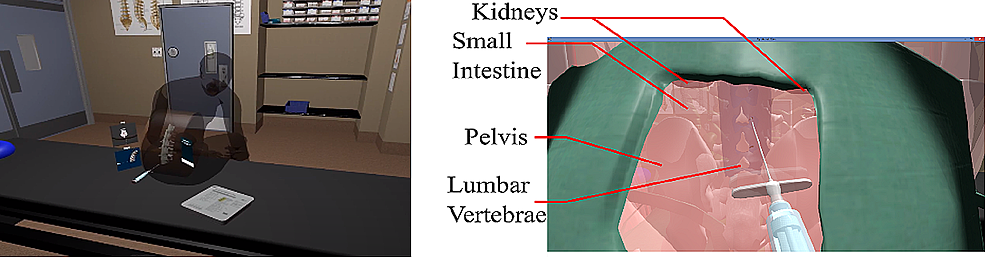
\includegraphics[width=0.7\linewidth]{capitulos/figuras/USEIT-visao-geral.png} 
    \caption{Ambiente virtual do USEIT \cite{Moo-Young2021}.}
    \label{fig:useitSimAmbienteVirtual}
\end{figure}

Um resumo das características importantes nos simuladores de anestesias regionais computacionais pode ser vista na Tabela \ref{tab:comparacaoSimuladoresComputacionais}.

\begin{sidewaystable}[!ht]
\begin{center}
\caption{Comparação dos simuladores computacionais.}
\label{tab:comparacaoSimuladoresComputacionais}
%\begin{tabular}{|p{0.27\linewidth}|p{0.55\linewidth}|p{0.105\linewidth}|}
\begin{tabular}{|c|c|c|c|c|c|c|c|c|c|c|}
\hline
  Nome do simulador & 
  \rotatebox{90}{Ano de desenvolvimento} & 
  \rotatebox{90}{Realidade virtual} & 
  \rotatebox{90}{Epidural (E) Raquianestesia (R)} & 
 \rotatebox{90}{Testado por especialistas} & 
  \rotatebox{90}{Baseado em dados medidos} & 
  \rotatebox{90}{Variabilidade de pacientes} & 
  \rotatebox{90}{Feedback para o usuário} & 
  \rotatebox{90}{Coluna palpável} & 
  \rotatebox{90}{Escolha do ponto de inserção da agulha }  & 
  \rotatebox{90}{Abordagens mediana (M) e paramediana (P)} \\
\hline\hline
 Epidural Sim & 1995 & 3D & E & S & S & Múltiplas & N & N & S & MP \\
 Epidural Injection Simulator Profile Manager & 2003 (1a versão) & 2D & E & N & N & Múltiplas & S & S & N &  \\
 Mediseus® epidural simulator & 2006 & 3D & E & S & N & 2 & N & N & N &  \\
 Spinal Anaesthesia simulator & 2006 & 3D & ER & N & S & Múltiplas & S & N & S & MP \\
 EpiSim & 2008 & 3D & E & N & N & Múltiplas & S & N & N &  \\
 Simulador de punção lombar de Färber & 2009 & 3D & ER  & S & S & 3 & S & N & S & MP \\
 Simulador epidural de Dubey & 2013 & 3D & E & N & S & Múltiplas & N & N & S & MP \\
 Epidural Haptic Game Simulator & 2017 & 3D & E & N & S & Múltiplas & S & N & S & MP \\
 Simulador epidural de Senac & 2019 & N & E & S & S & 3 & N & N & N &  \\
 USEIT & 2021 & 3D & E & N & N & 1 & S & N & S & MP \\
\hline
\end{tabular}
\end{center}
\end{sidewaystable}

\section {Comparação entre os simuladores estudados e o proposto nesta tese}
\label{sec:Comparacao}

Enquanto os simuladores baseados em \textit{phantom} mais generalistas possibilitam 4 variações de pacientes alguns dos simuladores computacionais mais completos possibilitam infinitas representações de pacientes através de ajustes de parâmetros \cite{Stredney1996, Wilson2003, N.2013, Brazil2017}. No simulador que desenvolvemos aqui também é possível configurar infinitas representações de pacientes como nestes simuladores. Isto é viabilizado pela adaptação do modelo 3D dinâmico que aumenta a espessura das camadas do corpo de acordo com os dados de \acrshort{IMC} passados como parâmetro ao sistema.  

Em contrapartida apenas um dos simuladores computacionais desenvolvidos tratou a apalpação física da coluna \cite{Wilson2003}. Esta é uma característica desejável e importante na raquianestesia que está presente em todos os simuladores baseados em \textit{phantoms}. O ambiente de treinamento desenvolvido nesta tese se aproxima da abordagem do simulador \textit{Epidural Injection Simulator, EIS} \cite{Wilson2003} no que diz respeito a esta característica, uma vez que apresenta através de interação com o dispositivo háptico a possibilidade de apalpação da coluna porém sem a necessidade do item físico. Tudo é feito através do uso do dispositivo háptico conectado e da \acrshort{RV}. Desta forma a limitação de escolha do ponto de inserção da agulha e sua angulação presente em \textit{Epidural Injection Simulator, EIS} não existe no simulador aqui proposto e esta é outra característica muito importante presente na maioria dos modelos baseados em \textit{phantoms}. Este fator já está incorporado também nos principais simuladores computacionais.

Um ponto positivo importante nos simuladores computacionais é se a representação do \textit{feedback} de forças na interação com os tecidos dos pacientes é baseada em dados medidos. Estes em alguns casos se baseiam em medições feitas em humanos ou animais mortos ou ainda em modelos matemáticos extraídos de exames de imagem de pacientes. Para este aspecto utilizamos nesta tese o mesmo modelo matemático baseado em dados de porcos e humanos como em \textcite{Brazil2017} porém, ao invés de fazer o uso de simplificações cilíndricas das camadas internas do corpo usados por ele, geramos um modelo 3D onde cada camada entre a pele e o último tecido alcançado é representado de forma fiel a anatomia do corpo humano. Para isto a modelagem destas camadas do tronco de um corpo feminino foi construída tomando como base um corpo 3D interativo e preciso do ponto de vista científico que está disponível para acesso público \cite{BioDigitalInc2019}. Desta forma chegamos a um resultado visual similar ao da visão 3D do simulador de punção lombar de Färber ou ainda do simulador USEIT sem a necessidade de fazer o uso de imagens médicas como em \textcite{Farber2009}. Ter uma representação correta das camadas internas do corpo na área de aplicação das punções é uma característica indispensável para que sejam corretamente adotadas as abordagens mediana e paramediana de inserção da agulha. O ambiente de treinamento que propomos aqui permite que as simulações destas duas abordagens sejam adotadas de forma que agulha atravesse as camadas corretas em cada caso. 

A possibilidade de se fazer infinitas simulações, característica inerente a todos os simuladores computacionais, também é uma grande vantagem destes. Em simuladores baseados em \textit{phantoms}, ao menos algumas peças têm as suas vidas úteis comprometidas com o grande número de procedimentos que precisam ser efetuados. São necessárias muitas repetições de procedimentos para que o médico adquira as habilidades das técnicas de anestesia de neuroeixo \cite{Konrad1998}. Pelo estudo de \textcite{Kopacz1996} são necessárias em torno de 45 procedimentos de raquidiana e 60 de peridural para que o iniciante chegue a 90\% de sucesso no procedimento. 

O \textit{feedback} para o usuário é outro ponto muito importante que somente pode ser implementado por simuladores computacionais. Dentre os simuladores estudados várias formas foram utilizadas para essas respostas como: gravações de execuções para estudo posterior \cite{Farber2009, Frazzetto2011}, a descrição do conhecimento obtido assim como a graduação da qualidade da prática \cite{Wilson2003, Albert2007, Dreifaldt2006, Brazil2017, Moo-Young202}. Estas características são fundamentais para uma ferramenta de aprendizado tanto para o aprendiz quanto para o avaliador. O aprendiz se beneficia ao acompanhar o seu aprendizado e pode aumentar sua dedicação em caso de identificação de falhas em algum ponto específico da prática. O avaliador pode usar o retorno da ferramenta para quantificar o nível de habilidade do aprendiz e definir limites antes da prática em pacientes reais. 

No ambiente de treinamento aqui desenvolvido apresentaremos diferentes níveis de dificuldade de procedimentos (no mínimo três) que precisam ser feitas com determinado nível de habilidade para que assim seja recebida uma nota geral de zero a dez relativo ao grau de assertividade do aprendiz na prática como um todo. Ele também receberá uma nota indicativa da habilidade demonstrada em cada nível e quais os pontos a melhorar (no caso de erros de procedimento serem identificados). A quantidade de procedimentos necessários de serem executados antes do sistema determinar que o desempenho do aprendiz foi satisfatório o que encerra o treinamento aumenta caso o aprendiz apresente muitos erros nos procedimentos e diminui com os procedimentos sendo feitos da forma correta o que de certa forma tem similaridades com outros simuladores que apresentam graduação da qualidade da prática. O \textit{Epidural Injection Simulator}, (EIS) desenvolvido por \textcite{Wilson2003} apresenta \textit{feedback} em tempo real e possibilita customização das forças e criação de cenários distintos dos inicialmente disponibilizados. O \textit{Spinal Anaesthesia Simulator} \cite{Albert2007,Dreifaldt2006} permite configuração de níveis de dificuldade e retorna para o usuário o nível de aprendizado e habilidades adquiridas em cada nível. O simulador desenvolvido por \textcite{Brazil2017thesis} também permite configuração das forças e atribui penalizações de acordo com os erros cometidos pelo aprendiz fornecendo desta forma um retorno que indica a evolução do aprendiz. No simulador USEIT é descrito como \textit{feedback} a sesanção de \acrshort{LoR} sentida ao pressionar a agulha adaptada ao háptico assim como métricas de avaliação do desempenho que não foram claramente detalhadas \cite{Moo-Young202}. 
